\documentclass[]{article}
\usepackage[version=3]{mhchem}
\usepackage{natbib}
\usepackage{graphicx}
\usepackage{float}
\bibliographystyle{abbrvnat}
\usepackage[colorlinks]{hyperref}
\hypersetup{
  citecolor = {blue},
}
\newcommand{\unit}[1]{\ensuremath{\, \mathrm{#1}}}

\title {Gas Density-Based Measurement of Biochemical Methane Potential (BMP)\footnote{
  Recommended citation: 
Hafner, S.D.; Astals, S.; Holliger, C.; Justesen, C.; Koch, K.; Mortensen, J.R. 2021 Gas density-based BMP measurement. Standard BMP Methods document 304, version 2.2. Available online: https://www.dbfz.de/en/BMP (accessed on March 31, 2021).
\newline
  Or see \url{https://www.dbfz.de/en/BMP} for a BibTeX file that can be imported into citation management software.
}
}
\author{Sasha D. Hafner, Sergi Astals, Christof Holliger, \\ Camilla Justesen, Konrad Koch, Jacob R. Mortensen, \\ S\"oren Weinrich} 

\date{\today \\
\bigskip
\textit{
  Document number 304.
  File version 2.2. 
  This document is from the Standard BMP Methods collection.
    \footnote{For more information and other documents, visit \url{https://www.dbfz.de/en/BMP}. 
    For document version history or to propose changes, visit \url{https://github.com/sashahafner/BMP-methods}.}
}
}

\begin{document}
\maketitle

\section{Introduction}
The gas density BMP (GD-BMP) method is an approach that does not require expensive gas analysis equipment needed for other manual biochemical methane potential (BMP) methods.
In this method, biogas volume and bottle mass loss are used together to determine biogas density, and from this, biogas composition is calculated.\footnote{Composition can only be determined from density when the a mixture contains two gases, \ce{CH4} and \ce{CO2} here.}
Together with biogas volume (or mass) measurements, methane (\ce{CH4}) production and BMP can be determined.
This document presents a detailed laboratory protocol needed for applying the GD-BMP method.
Development and validation of the method are described in \citet{justesenDevelopmentValidationLowcost2019}.
For information on GD-BMP calculations, see document 204 from the Standard BMP Methods website \citep{BMPdoc204gasdens}. 

\section{Equipment and supplies}
\label{sec:equipment}
For application of the GD-BMP method the following laboratory equipment and supplies are required:
\begin{itemize}
    \item Electronic scale
    \item Syringes and needles
    \item Manometer
    \item Typical BMP bottles and septa
    \item Incubator
\end{itemize}

The required accuracy of the scale will depend on the quantity of biogas produced. 
Generally, stated accuracy\footnote{
  Manufacturers often report accuracy as ``linearity''. 
  Note that accuracy is not the same as ``readability'', which is the smallest value that can be read. 
} of the scale should be at least 30 mg for every g of substrate volatile solids (VS) used.\footnote{
  For example, with 2 g of substrate VS added to each bottle, scale accuracy stated by the manufacturer must be 60 mg or better (e.g., 50 mg would be sufficient).
}
As described below, the accuracy and stability of the scale is checked as part of the protocol.

A simple closed U-tube manometer\footnote{
  A closed U-tube manometer can be made with plastic tubing filled with water and a simple valve made by folding some flexible tubing. See Fig. \ref{fig:utube} for an example.  
} or an inexpensive electronic manometer is sufficient for determining that post-venting headspace pressure is close to atmospheric before measuring volume.

For the highest precision in volume measurements for low or high biogas production, it is best to have several sizes of syringes for different interval measurements.
Ideally the largest syringe will be large enough to measure the largest volume of biogas produced in a single interval.\footnote{
\label{fn:cellrate}
  Biogas production rate depends on substrate and inoculum characteristics, and is best estimated from previous experiments.
  For microcrystalline cellulose plus inoculum, biogas production rate typically peaks around 200 mL g$^{-1}$ d$^{-1}$ (per g VS) within the first days, with values over 300 mL g$^{-1}$ d$^{-1}$ possible but rare (these values were taken from the data collected in the large IIS-BMP inter-laboratory study \citep{hafnerImprovingInterlaboratoryReproducibility2020}).
  With 2 g substrate VS then, syringe volume would ideally be more than 600 mL (300 $\times$ 2, perhaps 1 L), but a 150 mL syringe could be sufficient with multiple emptying cycles (see Section \ref{sec:volmeas}).
}
But large syringes are expensive.
Instead, a single small syringe can be used multiple times to remove the biogas from a single bottle in a single interval.
However, this approach requires a valve in addition to a manometer and it is slightly more complicated (see Section \ref{sec:volmeas} for details).

An incubator or temperature-controlled room is needed to keep bottles at the desired test temperature, e.g., 37 $^\circ$C.
A water bath is not recommended because water on a bottle surface will affect its weight.
Incubation of the bottles in heated air is preferable.
Ideally, venting and weighing should be done inside a temperature-controlled room, so bottles are always at the incubation temperature and the headspace temperature -- needed for calculations -- is known.
However, the effect of headspace temperature error on accuracy is very small, so this is not required.
A mechanical mixer is not needed; careful manual mixing at the time of sampling has been found to be sufficient (see Section \ref{sec:incsam}).\footnote{But gentle mechanical mixing could work, as long as the inside of the septum is kept clean.}

\section{Setup}
\label{sec:setup}
During setup, inoculum and substrate are added to bottles, and the headspace of each bottle is flushed to remove \ce{O2} and ensure anaerobic conditions. 
Bottles are then weighed and placed in an incubator.
Setup should follow the requirements listed in document 100 \citep{BMPdoc100req}, including the use of a positive control\footnote{Microcrystalline cellulose is required currently, but if it is unavailable, other common substrates may be useful; see \citet{kochEvaluationCommonSupermarket2020} for suggestions. But note that BMP can not be validated without microcrystalline cellulose at this time \citep{BMPdoc100req}.}
and at least 3 replicates for each substrate.

\subsection{Inoculum and substrate quantities and bottle size}
\label{sec:quantities}
Selecting quantities of inoculum and substrate, as well as bottle size (volume) is typically based on experience.
Some general guidance is given here; these suggested values can be adjusted depending on results and substrate characteristics.

The GD-BMP method requires determination of small mass losses from a heavy BMP bottle, so in general, maintaining high mass loss should be a goal.
Therefore, substrate mass should generally be at least 1 g VS.
Starting with this value as a minimum, inoculum quantity can be determined based on inoculum-to-substrate ratio (ISR), which is expressed on a VS basis and should generally be 2:1.\footnote{See \citet{holligerStandardizationBiomethanePotential2016} for more discussion on this topic.}

With substrate and inoculum quantities, a bottle size can be selected.
Alternatively, given a bottle size, the largest possible quantities can be selected.
The accuracy of the GD-BMP method is affected only slightly by variation in headspace pressure, and it is possible to correct for leakage of biogas. 
However, for safety (to avoid exploding bottles), for maximum precision, and to minimize possible (but perhaps unlikely) effects of high \ce{CO2} dissolution, headspace pressure should be kept below 200 kPa (2 bar) gauge pressure, or even more cautiously, 100 kPa \citep{hafnerSystematicErrorManometric2019}. 
Bottle pressures can be estimated from headspace volume and expected (or measured) biogas volume.
The headspace volume can be estimated by assuming a density of 1 mL g$^{-1}$ for the mixture.
Additionally, to minimize the risk of foaming causing contamination of the septum, bottles are typically not filled beyond 50\%.

Using the information given in note \ref{fn:cellrate} for cellulose (maximum peak biogas production typically around 200 but possibly as high as 300 mL g$^{-1}$ d$^{-1}$) and the maximum recommended headspace pressures given above, headspace volume should between 100 and 300 mL per g substrate VS.
This target can be adjusted based on expected degradation rate and biogas potential, i.e., slower, faster, or similar biogas production compared to cellulose.
But error from initial headspace\footnote{Due to a difference in density between the flushing gas and biogas.} increases with the ratio of headspace volume to total biogas production, and although a correction is available \citep{justesenDevelopmentValidationLowcost2019}, it is less accurate when residual flushing gas remains in the headspace.
Therefore headspace volumes above 300 mL g$^{-1}$ should be avoided if possible.

The ``planning'' tool in the web app OBA is helpful for quickly calculating substrate and inoculum quantities: \url{https://biotransformers.shinyapps.io/oba1/}.
This tool also checks values against the recommendations given in \citet{holligerStandardizationBiomethanePotential2016}.
Three examples for three different bottle sizes that meet the recommendations given in \citet{holligerStandardizationBiomethanePotential2016} in addition to the GD-BMP recommendations given in this section are shown in Table \ref{tab:examples} below.

\begin{table}[h] 
\centering
\caption{Example quantity and volume information for three bottle sizes for GD-BMP method. Note that for example C, it would not be possible to meet all recommendations if the inoculum had a VS concentration below 3.4\%.}
\label{tab:examples}
\begin{tabular}{llll}
\hline
Parameter                     & A    & B   & C   \\
\hline
Total bottle volume (mL)      & 520  & 250 & 160 \\
Inoculum VS (\% FM)           & 2.0  & 2.0 & 4.0 \\
Substrate VS (\% FM)          & 99   & 99  & 99  \\
ISR (VS basis)                & 2.0  & 2.0 & 2.0 \\
Substrate VS (g)              & 1.50 & 1.0 & 1.0 \\
Inoculum FM (g)               & 150  & 101 & 50  \\
Substrate FM (g)              & 1.52 & 1.0 & 1.0 \\
Mixture FM (g)                & 152  & 101 & 51  \\
Headspace volume (mL)         & 368  & 149 & 109 \\
Headspace:substrate VS (mL:g) & 245  & 149 & 109 \\
\hline
\end{tabular}
\end{table}

\subsection{Step-by-step instructions}
\begin{enumerate}
  \item Carefully set up and level the scale on a stable surface (following manufacturer's instructions) and check its accuracy with a weight set. 
      It is particularly important that the actual accuracy is close to reported accuracy when weighing an object with a mass close to the total mass of a BMP bottle and its contents. 
      For a scale with a reported accuracy of 50 mg, for example, this could be checked by taring the scale with a full bottle or equivalent mass, and adding a 50 mg scale calibration weight.
      Problems with accuracy or stability over time could be related to air currents, and can generally be addressed by selecting a proper location or blocking air flow with, e.g., a cardboard box.
    \item Add the required mass of inoculum and substrate (see Section \ref{sec:quantities}), along with any other additions (e.g., a trace element solution \citep{holligerStandardizationBiomethanePotential2016}) to each labeled bottle and seal with a septum and cover. 
      Determination of the quantity of material added by mass difference is the recommended approach: tare scale with bottle, add approximately the desired quantity, wipe any material from near the mouth of the bottle, and finally determine the actual quantity from the scale reading. 
      Note that the scale used here does not need to be the same scale used for determining mass loss (see Section \ref{sec:incsam}).
    \item Flush the bottle headspace to remove \ce{O2}. 
      A simple approach is to use a needle attached to a flow meter (e.g., a rotameter), a pressure regulator (to ensure low pressure), and a gas cylinder with plastic tubing, along with a separate needle for venting. With the GD-BMP method, pure \ce{N2} is preferred for flushing over \ce{N2}/\ce{CO2} mixtures.\footnote{
        Flushing gas results in an (generally small) error because its density may differ from produced biogas density (the density of \ce{N2} is identical to a \ce{CH4}:\ce{CO2} mixture with 58\% \ce{CH4} and 42\% \ce{CO2}) but this can be corrected in calculations \citep{justesenDevelopmentValidationLowcost2019}.
} 
      Minimize \ce{CO2} stripping by flushing for only 3 to 4 headspace volume exchanges. 
      Ensure that the flushing gas does not bubble through the liquid in the bottle (needle should not be submerged) to avoid \ce{CO2} stripping. 
      Allow the pressure in each bottle’s headspace to equilibrate with atmospheric pressure before removing the venting needle.
    \item Make 3 ``control'' bottles to use to to check the stability of the scale
      It is essential that they have constant mass throughout the experiment. 
      Ideally they should be a similar size and weigh about as much as the other BMP bottles.
      This can be done by adding dry sand to a BMP bottle and sealing the top with a septum. 
      Bottles filled with water have been used successfully, but in other cases have been found to lose a small amount of water.  
      Calibration weights for scales could also be used.
    \item Weigh each bottle and record as ``initial mass''. 
      Repeat this initial weighing in order to minimize the chance of a recording error, because calculations of cumulative \ce{CH4} production at all timepoints require an accurate initial mass measurement.
      If there is a discrepancy between these two initial measurements, weigh again to determine the correct mass.
      It is important that the only change in bottle mass after this time is due to biogas removal.
      Bottles should be kept clean, and labels should not be added after this time, for example.
    \item Place bottles in the incubator set at the test temperature.
\end{enumerate}

\section{Incubation and sampling}
\label{sec:incsam}
Bottles are removed from the incubator occasionally to vent and weigh in what is here referred to as a ``sampling event''.
Details on sampling frequency can be found in Section \ref{sec:freq} and step-by-step instructions for each event in Section \ref{sec:steps}.
Biogas temperature affects water vapor content. 
To minimize uncertainty in the headspace temperature used in calculations, the time that bottles spend outside the incubator should be as short as possible, and the same procedure and timing should be followed for each sampling event. 

Unlike headspace conditions, it is important to determine the temperature and pressure of biogas at the time of each measurement in order to standardize the volume.
When using syringes, it is reasonable to assume that the syringe and gas inside are approximately at ambient temperature.
With a manometer, the pressure can be kept nearly identical to the ambient value.
Therefore ambient pressure and temperature (room pressure and temperature) must be determined or, if necessary, estimated.
Absolute pressure can now be measured using barometer apps on many smart phones, which can also be used for temperature measurement in conjunction with an external sensor.
Alternatively, pressure can be determined from public meteorological data (from a nearby weather station), with corrections for elevation if necessary.

\subsection{Sampling frequency}
\label{sec:freq}

Determining when to sample bottles in any manual BMP method, i.e., when to intermittently remove and measure accumulated biogas, is typically based on experience. 
Some general considerations are:
\begin{itemize}
	\item As long as the headspace:substrate VS ratio is sufficiently high (see Section \ref{sec:quantities}), there is no need to sample more than once per day
  \item Sampling frequency can change over time, and is generally highest at the start (1 d interval) and low at the end (maximum of perhaps a 7 d interval)
  \item As long as biogas is not lost before or during measurement due to leakage, sampling frequency does not strongly affect accuracy or precision of the GD-BMP method
\end{itemize}

Following these recommendations, a good approach is to sample daily from the start, and reduce the sampling frequency as biogas production slows, taking care to avoid high headspace pressure or too much accumulated biogas for the sampling system.

\subsection{Biogas volume measurement}
\label{sec:volmeas}
Biogas volume measurement in Section \ref{sec:steps} should take place at ambient pressure, in order to later convert the measurement to standardized volume.
This task can be done very simply with an inexpensive plastic syringe and a simple U-tube manometer, as long as the capacity of the syringe (maximum volume) is greater than the quantity of biogas produced in any sampling interval.
Unfortunately, typical plastic syringes are generally not large enough ($\le$ 150 mL), and large syringes (e.g., 1 L) are expensive.
There are at least two solutions:
\begin{itemize}
  \item Use multiple syringes to remove accumulated gas all at one time. %hedgehog hehehe   CAJU: What is this comment? SDH: Sergi's multi-syringe monster :)
  \item Use a manometer and a valve to measure accumulated gas in steps. 
\end{itemize}

The first approach is straightforward, but handling three or more syringes with only two hands is challenging.
The second requires a valve and a manometer, and one possible implementation is shown in Fig. \ref{fig:utube}.
Its construction and use is described here.
In this section the capital letters (labeled with A, B, C) and small Greek letters ($\alpha$, $\beta$, ...) refer to the labels in Fig. \ref{fig:utube}.
A manometer can be made from flexible plastic tubing, large enough to avoid problems due to adhesion.\footnote{Clear polyvinyl chloride (PVC) tubing with a 10 mm (3/8 inch) inner diameter works well.}
It is filled with water to the level shown by $\beta$, and clamped at location $\alpha$ to create a \textit{closed}-tube manometer.
Clamping is essential; an open-tube manometer would lose its water under even moderate pressure.
Smaller diameter tubing (at $\gamma$) can be used to connect to the three-way valve (A, B, C in Fig. \ref{fig:utube}).\footnote{Plastic valves sometimes called "disposable medical three-way stopcock valves" are inexpensive and work well for this task.}
When in use, the system is connected to a BMP bottle via a needle ($\delta$).\footnote{21 gauge/0.8 mm works well.}
A syringe is connected through tubing to the valve ($\varepsilon$).
This connection should be easy to disconnect, in order to vent biogas.
With this system, the following steps are used for each bottle.

\begin{enumerate}
  \item With syringe disconnected (around location $\varepsilon$), check that water levels at $\beta$ are equal. Equilibrate closed end by removing and replacing clamp at $\alpha$ if necessary.
  \item Turn valve so connection B-C is open (A closed) and allow accumulated biogas to flow under pressure to no more than 80\% of syringe capacity.
  \item Turn valve so connection A-C is open (B closed) and adjust syringe plunger position so the water levels at $\beta$ are equal. Read and record volume.
  \item Disconnect syringe at $\varepsilon$, push out biogas, and return to step 1, repeating until all excess accumulated biogas has been removed, i.e., when headspace pressure is equal to atmospheric (determined by opening A-B, or even A-B-C if possible).
\end{enumerate}

For an even simpler system, a regular (two-way) valve (possibly clamped tubing) could be place between the syringe and bottle (needle), with a manometer attached directly to the syringe.

\begin{figure}
  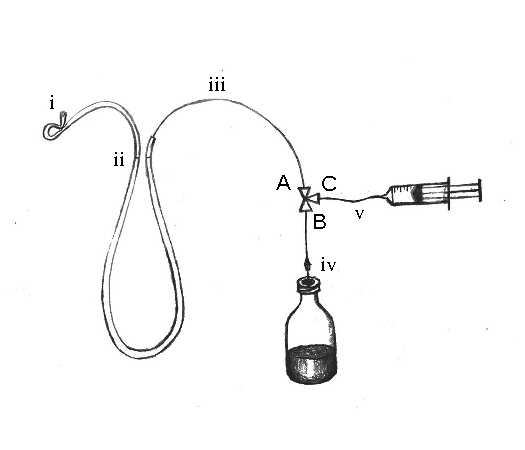
\includegraphics[]{figs/GD_utube.pdf}
  \caption{The U-tube manometer/3-way valve approach to measure biogas volume. The dashed line surrounds the u-tube manometer, which could be replaced with a digital model. See Section \ref{sec:volmeas} for a detailed explanation.} 
  \label{fig:utube}
\end{figure}

\subsection{Step-by-step instructions} 
\label{sec:steps}
\begin{enumerate}
    \item Measure and record the room temperature and pressure at which biogas volume will be determined.
    \item Remove the 3 control bottles from the incubator and weigh them to confirm scale consistency. 
      If the results are the same as the initial masses (within the expected accuracy) proceed, otherwise, identify and address the problem with the scale or replace the scale if necessary.
      If the problem cannot be resolved, proceed and later correct mass results for scale drift.\footnote{
        Correction is done by subtracting the average apparent mass gain in the control bottles from all mass measurements made during that particular sampling event. 
        For example, if both water controls weighed 0.1 g more on day 4 than at the start, the measured masses of \textit{all} bottles from day 4 should be adjusted downward by 0.1 g.
      }
    \item Remove a single set of replicates from the incubator (e.g., the three replicates for cellulose).
    \item Always starting with the same replicate (e.g., ``1'' or ``a''),\footnote{
        If this is done, the effect of gradual headspace cooling on measurement error (expected to be minor) can be confirmed by comparing BMP from individual replicates across all substrates.
      } gently swirl (not shake) the bottle for at least 10 s to mix the contents and encourage \ce{CO2} equilibration between solution and headspace. 
      During swirling, avoid contact between the liquid and the septum to prevent mass losses.\footnote{
        If the septum becomes contaminated with reacting material, a small amount may be pushed out during venting, which will result in error in the determination of mass loss.
        Generally it is easy to avoid this problem, but if it does occur, be sure to note the occurrence to help with interpretation later.
        If the loss is small and there is no noticeable difference among the replicates, the problem could be ignored. 
        Otherwise, data from this replicate should be discarded.
      }
    \item Weigh the bottle and record the result as pre-venting mass.
    \item Vent the bottle using a syringe and measure biogas volume (see Section \ref{sec:volmeas}). Prevent the needle from contacting any reacting material; keep it in the gas phase. 
      Use the manometer to ensure that the pressure of both biogas in the syringe and biogas remaining in the bottle headspace after venting pressure is close to atmospheric (gauge pressure = 0 $\pm3 $ kPa).
    \item Weigh the bottle after venting, and record the result as post-venting mass. 
    \item Proceed to the next replicate (e.g., ``2'' or ``b'') and repeat steps 4 to 7.
    \item After all replicates have been mixed, weighed, vented, and weighed again, place the bottles back in the incubator.
    \item Proceed to the next set of replicates (e.g., the three replicates for substrate ``food waste A'') and repeat steps 3 to 9.
\end{enumerate}

This sequence of steps is shown in Fig. \ref{fig:steps}.

\begin{figure}[ht]
  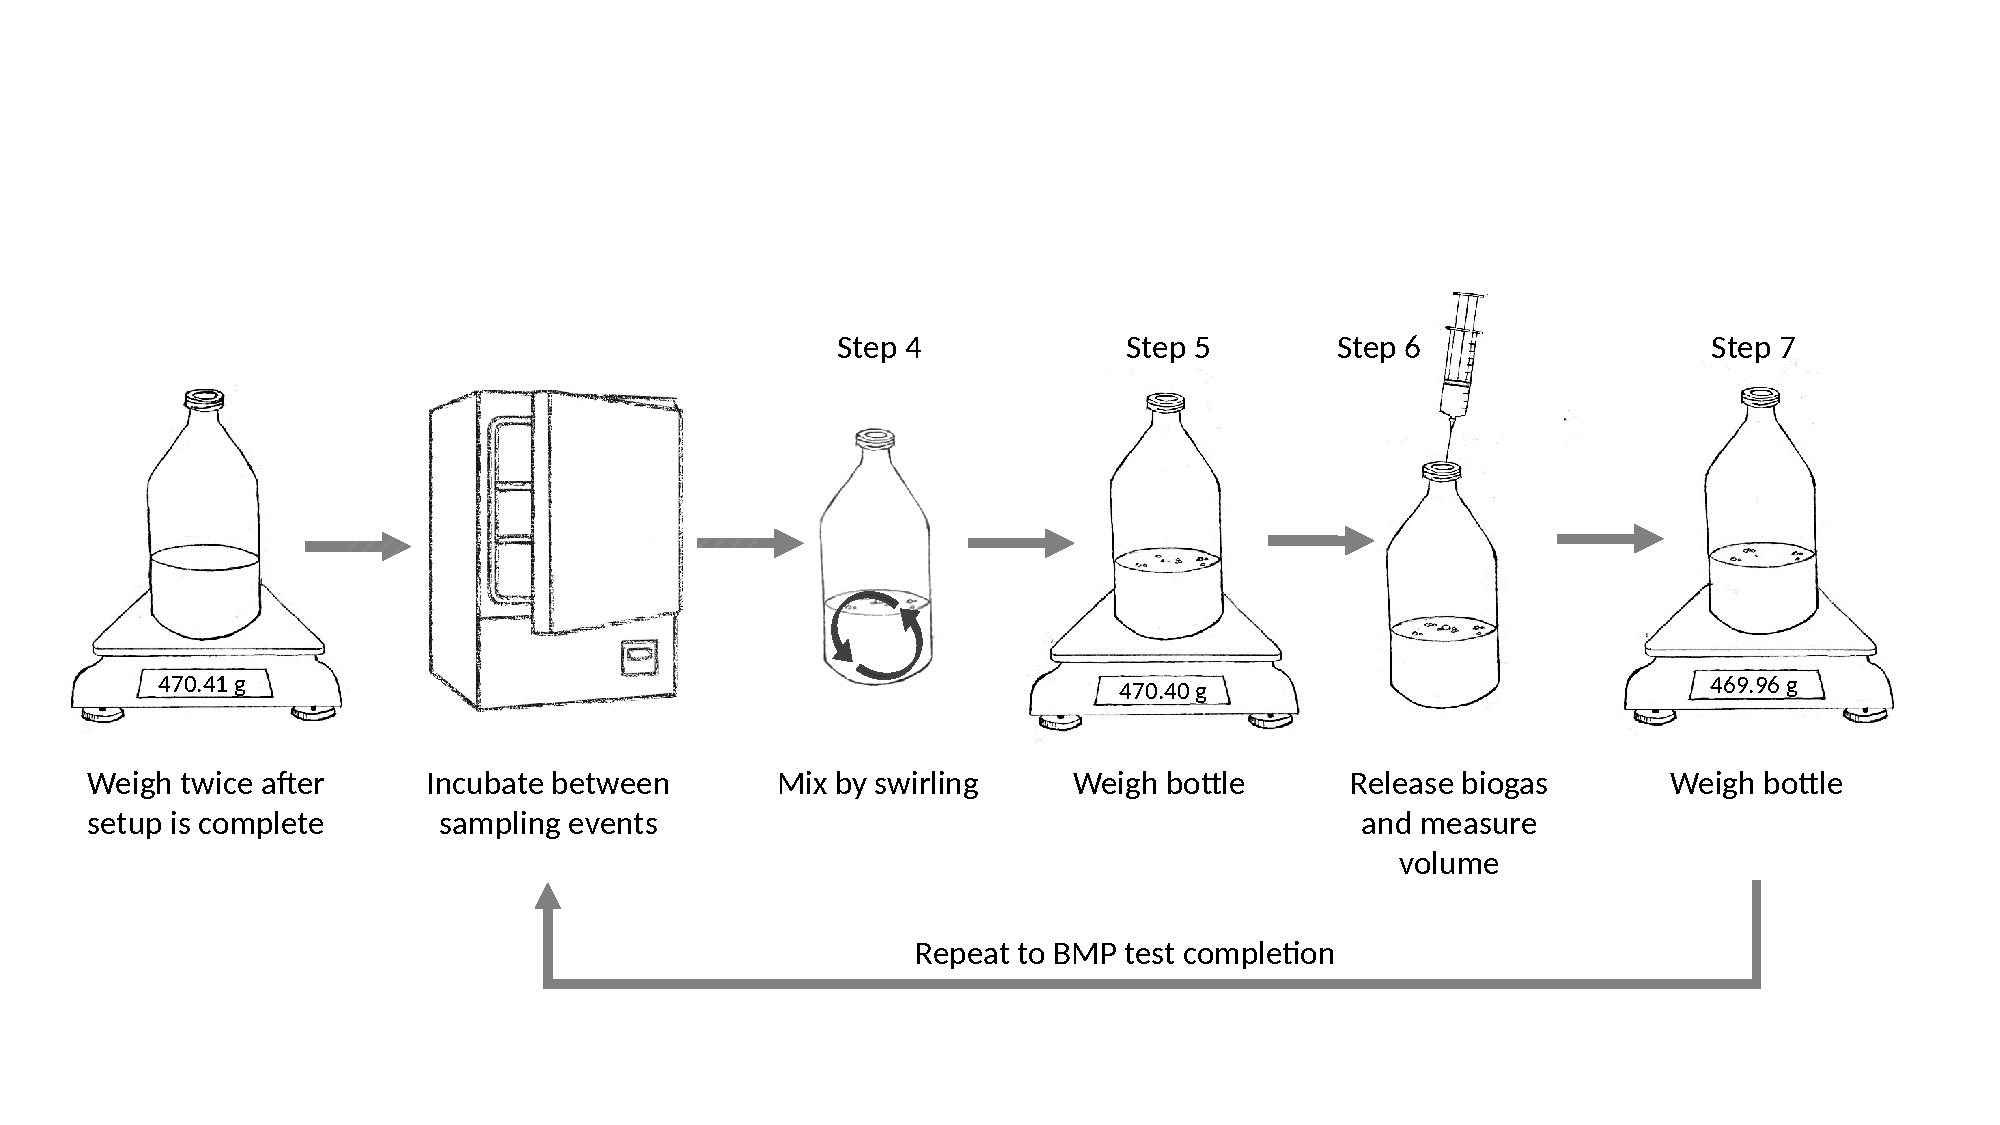
\includegraphics[width=\textwidth]{figs/GD_steps.pdf}
  \caption{The data collection steps required for GD-BMP measurements. Step numbers match those listed in the text, and are repeated for each sampling event. For details on volume measurement (step 6) see Section \ref{sec:volmeas}.}
  \label{fig:steps}
\end{figure}


\section{Testing}
The GD-BMP method requires accurate determination of gas volume and bottle mass loss.
It is important that any new setup is tested.
Fortunately, ambient air can be used as a standard.
To test the system, simply use a syringe to \textit{carefully} force a volume (it is difficult to add more than about 20\% of a bottle headspace) into an empty bottle, and proceed with the measurement steps given above. 
Calculate apparent density based on bottle mass loss and volume of gas removed.\footnote{This volume is typically smaller than the volume thought to be added because of leakage during addition or removal of the syringe.}
The value should be within 10\% (or better, 5\%) of the density for the known ambient pressure and temperature.\footnote{Air density can be calculated with \url{https://www.density.co.uk/calculators/density-of-air/} or similar tools. Humidity effects are small around room temperature (assuming temperature $\le$ 25$^\circ$C). Density is 1.20 mg mL$^{-1}$ for dry air at 20$^\circ$C and 101.3 kPa, and 1.19 mg mL$^{-1}$ when saturated with water.}

\section{Calculations}
See document 204 from the Standard BMP Methods website \citep{BMPdoc204gasdens} for a detailed description of calculations for the GD-BMP method.
Calculations can also be carried out using the free web app OBA (\url{https://biotransformers.shinyapps.io/oba1/}) or the biogas package in R (\url{https://cran.r-project.org/package=biogas}) \citep{hafnerSoftwareBiogasResearch2018}.
Final results should always be evaluated based on current validation criteria \citep{BMPdoc100req}.

\bibliography{bib}

\end{document}
